\chapter{Kleurgebaseerde similariteitsmaten}

In dit hoofdstuk construeren we enkele similariteitsmaten die beelden 
vergelijken op basis van de kleuren die er in voorkomen. We identificeren de beelden
in dit geval dus met vaagverzamelingen in een universum dat bestaat uit kleuren 
in plaats van beeldpunten. Vermits kleur \'e\'en  van de meest gebruikte kenmerken is bij CBIR 
\cite{rui:image_retr, schettini:survey_of_methods_for_colour_image_indexing_and_retrieval}, mogen we 
verwachten dat die \emph{kleurgebaseerde} aanpak effici\"ente 
similariteitsmaten zal opleveren. 

\section{Histogrammen}

Een \emph{histogram} van een kleurbeeld is een voorstelling van de frequentieverdeling 
van de verschillende kleuren. De waarde van het histogram voor een kleurbeeld 
$A$ in de kleur $c \in C$ is dus gelijk aan het totaal aantal pixels in het beeld met 
kleur $c$. Om de complexiteit te beperken wordt er in de praktijk gebruik gemaakt
van kleurkwantisatie. Het universum der kleuren $C$ wordt dus beperkt tot $C' \subset C$. 
%Het histogram wordt dus berekend voor verzamelingen van
%kleuren in plaats van individuele kleuren. 
De waarde van het histogram voor een beeld $A$ in de kleur $c \in C'$ is dan gelijk aan 
het totaal aantal pixels in $A$ die tot bin $bin(c)$ behoren. Met andere woorden: het histogram 
geeft de frequentieverdeling weer van de kleuren uit $C'$ in de gekwantiseerde versie van 
$A$. We noteren de waarde in $c$ van het histogram van een beeld $A$ met $h_A(c)$: 
$$ 
h_A(c) = \sum_{p \in P} \delta (bin(c) - bin(A(p))) 
$$ 
waarbij $\delta$ de Diracfuntie is en $P$ het universum der beelpunten 
voorstelt. De functie $bin$ is uiteraard de $C - \{1,2,\ldots,N\}$ afbeelding 
uit \ref{sectie:kleurkwantisatie}, die met 
elke kleur het nummer van \'e\'en van de $N$ bins associeert. 


\subsection{Pseudo-vage histogrammen}

Door de waarden van een histogram te normaliseren, kunnen we het omzetten naar 
een vaagverzameling in het universum der kleuren $C'$ 
\cite{debaets:similariteitsmaten_voor_kleurbeelden, vanderweken:similariteitsmaten, vertan:embedding_fuzzy_logic_in_cbir}. 
Dat houdt in dat we elke 
waarde van het histogram delen door het maximaal aantal pixels met dezelfde 
kleur. We hebben dus de volgende uitdrukking voor de lidmaatschapsgraad van de 
kleur $c \in C$ in de vaagverzameling $H_A$ geassocieerd met het histogram 
van beeld $A$: 
$$
H_A(c) = \frac{\displaystyle h_A(c)}{\displaystyle \max_{c \in C'}(h_A(c))}
$$ 
Een dergelijke vaagverzameling noemen we een \emph{pseudo-vaag histogram}. 
De kleur die het meest voorkomt heeft daarbij lidmaatschapsgraad $1$. Alle 
andere kleuren hebben kleinere lidmaatschapsgraden. 

We beschouwen de zes uniforme en de eerste twee niet-uniforme (focale kleuren en SCT) 
kwantisatietechnieken uit \ref{sectie:kleurkwantisatie}. Figuur~\ref{fig:histogrammen_eerste_vb} bevat
de pseudo-vage histogrammen die we zo bekomen voor het ``geel bootje'' voorbeeld
uit onze testcollectie. In figuur~\ref{fig:alle_histn_geel_bootje} worden de pseudo-vage histogrammen
getoond van alle beelden uit de testcollectie die relevant zijn ten opzichte van dat voorbeeld.

\begin{figure}[!t]
\begin{center}
\begin{tabular}{c}
\subfigure[] {
\begin{minipage}[c]{0.3\textwidth}
\begin{center}
\includegraphics[height=2.7cm, width=\textwidth]{images/hist_hsv_obj3__0.eps}
\end{center}
\vspace{2pt}
\end{minipage}
}
\subfigure[] {
\begin{minipage}[c]{0.3\textwidth}
\begin{center}
\includegraphics[height=2.7cm, width=\textwidth]{images/hist_irb_obj3__0.eps}
\end{center}
\vspace{2pt}
\end{minipage}
}
\subfigure[] {
\begin{minipage}[c]{0.3\textwidth}
\begin{center}
\includegraphics[height=2.7cm, width=\textwidth]{images/hist_i1i2i3_obj3__0.eps}
\end{center}
\vspace{2pt}
\end{minipage}
}\\
\subfigure[] {
\begin{minipage}[c]{0.3\textwidth}
\begin{center}
\includegraphics[height=2.7cm, width=\textwidth]{images/hist_xyz_obj3__0.eps}
\end{center}
\vspace{2pt}
\end{minipage}
}
\subfigure[] {
\begin{minipage}[c]{0.3\textwidth}
\begin{center}
\includegraphics[height=2.7cm, width=\textwidth]{images/hist_yxy_obj3__0.eps}
\end{center}
\vspace{2pt}
\end{minipage}
}
\subfigure[] {
\begin{minipage}[c]{0.3\textwidth}
\begin{center}
\includegraphics[height=2.7cm, width=\textwidth]{images/hist_lab_obj3__0.eps}
\end{center}
\vspace{2pt}
\end{minipage}
}\\
\subfigure[] {
\begin{minipage}[c]{0.1\textwidth}
\begin{center}
\includegraphics[height=2.7cm, width=\textwidth]{images/hist_focal_obj3__0.eps}
\end{center}
\vspace{2pt}
\end{minipage}
}
\subfigure[] {
\begin{minipage}[c]{0.3\textwidth}
\begin{center}
\includegraphics[height=2.7cm, width=\textwidth]{images/hist_sct_obj3__0.eps}
\end{center}
\vspace{2pt}
\end{minipage}
}
\subfigure[] {
\begin{minipage}[c]{0.5\textwidth}
\begin{center}
\includegraphics[height=2.7cm, width=\textwidth]{images/hist_fuzzy_obj3__0.eps}
\end{center}
\vspace{2pt}
\end{minipage}
\label{fig:vaaghistogram_eerste_vb}
}
\end{tabular}
\caption{\label{fig:histogrammen_eerste_vb}De verschillende histogrammen voor het ``geel bootje'' 
voorbeeld (HSV (a), Irb (b), I1I2I3 (c), XYZ (d), Yxy (e) en L*a*b* (f), focale kleuren (g), SCT (h) 
en het vaaghistogram voor $\lambda = 5$ (i)).}
\end{center}
\end{figure}

\begin{figure}[tbp]
\begin{center}
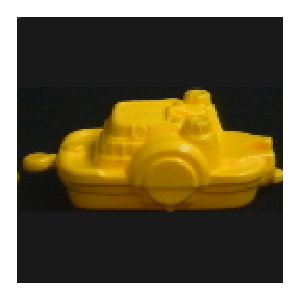
\includegraphics[width=2.5cm]{coil/beeld-12.eps}
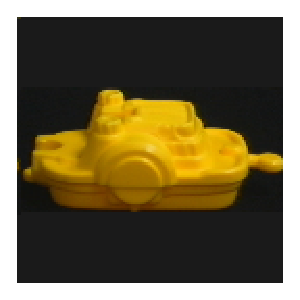
\includegraphics[width=2.5cm]{coil/beeld-13.eps}
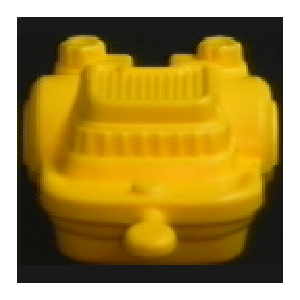
\includegraphics[width=2.5cm]{coil/beeld-14.eps}
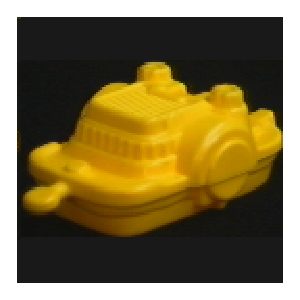
\includegraphics[width=2.5cm]{coil/beeld-15.eps}
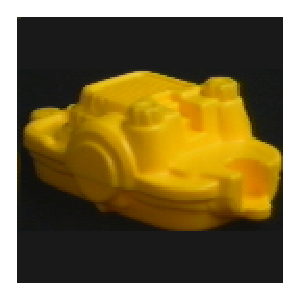
\includegraphics[width=2.5cm]{coil/beeld-16.eps}
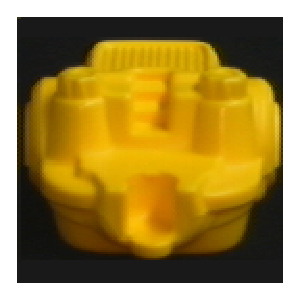
\includegraphics[width=2.5cm]{coil/beeld-17.eps}\\[5pt]
\includegraphics[width=2.5cm]{images/hist_hsv_obj3__0.eps}
\includegraphics[width=2.5cm]{images/hist_hsv_obj3__45.eps}
\includegraphics[width=2.5cm]{images/hist_hsv_obj3__90.eps}
\includegraphics[width=2.5cm]{images/hist_hsv_obj3__180.eps}
\includegraphics[width=2.5cm]{images/hist_hsv_obj3__270.eps}
\includegraphics[width=2.5cm]{images/hist_hsv_obj3__315.eps}\\[5pt]
\includegraphics[width=2.5cm]{images/hist_irb_obj3__0.eps}
\includegraphics[width=2.5cm]{images/hist_irb_obj3__45.eps}
\includegraphics[width=2.5cm]{images/hist_irb_obj3__90.eps}
\includegraphics[width=2.5cm]{images/hist_irb_obj3__180.eps}
\includegraphics[width=2.5cm]{images/hist_irb_obj3__270.eps}
\includegraphics[width=2.5cm]{images/hist_irb_obj3__315.eps}\\[5pt]
\includegraphics[width=2.5cm]{images/hist_i1i2i3_obj3__0.eps}
\includegraphics[width=2.5cm]{images/hist_i1i2i3_obj3__45.eps}
\includegraphics[width=2.5cm]{images/hist_i1i2i3_obj3__90.eps}
\includegraphics[width=2.5cm]{images/hist_i1i2i3_obj3__180.eps}
\includegraphics[width=2.5cm]{images/hist_i1i2i3_obj3__270.eps}
\includegraphics[width=2.5cm]{images/hist_i1i2i3_obj3__315.eps}\\[5pt]
\includegraphics[width=2.5cm]{images/hist_xyz_obj3__0.eps}
\includegraphics[width=2.5cm]{images/hist_xyz_obj3__45.eps}
\includegraphics[width=2.5cm]{images/hist_xyz_obj3__90.eps}
\includegraphics[width=2.5cm]{images/hist_xyz_obj3__180.eps}
\includegraphics[width=2.5cm]{images/hist_xyz_obj3__270.eps}
\includegraphics[width=2.5cm]{images/hist_xyz_obj3__315.eps}\\[5pt]
\includegraphics[width=2.5cm]{images/hist_yxy_obj3__0.eps}
\includegraphics[width=2.5cm]{images/hist_yxy_obj3__45.eps}
\includegraphics[width=2.5cm]{images/hist_yxy_obj3__90.eps}
\includegraphics[width=2.5cm]{images/hist_yxy_obj3__180.eps}
\includegraphics[width=2.5cm]{images/hist_yxy_obj3__270.eps}
\includegraphics[width=2.5cm]{images/hist_yxy_obj3__315.eps}\\[5pt]
\includegraphics[width=2.5cm]{images/hist_lab_obj3__0.eps}
\includegraphics[width=2.5cm]{images/hist_lab_obj3__45.eps}
\includegraphics[width=2.5cm]{images/hist_lab_obj3__90.eps}
\includegraphics[width=2.5cm]{images/hist_lab_obj3__180.eps}
\includegraphics[width=2.5cm]{images/hist_lab_obj3__270.eps}
\includegraphics[width=2.5cm]{images/hist_lab_obj3__315.eps}\\
\includegraphics[width=1cm,height=2.5cm,angle=-90]{images/hist_focal_obj3__0.eps}
\includegraphics[width=1cm,height=2.5cm,angle=-90]{images/hist_focal_obj3__45.eps}
\includegraphics[width=1cm,height=2.5cm,angle=-90]{images/hist_focal_obj3__90.eps}
\includegraphics[width=1cm,height=2.5cm,angle=-90]{images/hist_focal_obj3__180.eps}
\includegraphics[width=1cm,height=2.5cm,angle=-90]{images/hist_focal_obj3__270.eps}
\includegraphics[width=1cm,height=2.5cm,angle=-90]{images/hist_focal_obj3__315.eps}\\[5pt]
\includegraphics[width=2.5cm]{images/hist_sct_obj3__0.eps}
\includegraphics[width=2.5cm]{images/hist_sct_obj3__45.eps}
\includegraphics[width=2.5cm]{images/hist_sct_obj3__90.eps}
\includegraphics[width=2.5cm]{images/hist_sct_obj3__180.eps}
\includegraphics[width=2.5cm]{images/hist_sct_obj3__270.eps}
\includegraphics[width=2.5cm]{images/hist_sct_obj3__315.eps}
\caption{\label{fig:alle_histn_geel_bootje}De verschillende pseudo-vage histogrammen voor de beelden 
van het geel bootje.}
\end{center}
\end{figure}

\begin{figure}[tbp]
\begin{center}
\includegraphics[height=2cm]{coil/beeld-12.eps}
\includegraphics[height=2cm]{images/hist_fuzzy_obj3__0.eps}\hspace{1cm}
\includegraphics[height=2cm]{coil/beeld-13.eps}
\includegraphics[height=2cm]{images/hist_fuzzy_obj3__45.eps}\\[5pt]
\includegraphics[height=2cm]{coil/beeld-14.eps}
\includegraphics[height=2cm]{images/hist_fuzzy_obj3__90.eps}\hspace{1cm}
\includegraphics[height=2cm]{coil/beeld-15.eps}
\includegraphics[height=2cm]{images/hist_fuzzy_obj3__180.eps}\\[5pt]
\includegraphics[height=2cm]{coil/beeld-12.eps}
\includegraphics[height=2cm]{images/hist_fuzzy_obj3__270.eps}\hspace{1cm}
\includegraphics[height=2cm]{coil/beeld-12.eps}
\includegraphics[height=2cm]{images/hist_fuzzy_obj3__315.eps}
\caption{\label{fig:alle_vaaghistn_geel_bootje}De verschillende vaaghistogrammen voor de beelden 
van het geel bootje.}
\end{center}
\end{figure}

%Voor een RGB-beeld gebruikt men typisch 8 bits per kleurcomponent. Dit geeft een totaal van
%24 bits per kleur, zodat men dus $2^{24}=2^4 \cdot 2^{20}=16 \cdot 2^{20} \approx 16 \cdot 10^6$
%kleuren kan voorstellen. Een genormaliseerd histogram bestaat dan dus uit 16 miljoen waarden.
%Similariteitsmaten op basis van dergelijke histogrammen zouden dus veel te veel rekentijd vragen.

\subsection{Vaaghistogrammen}

Naast de bovenstaande vage interpretatie van het klassieke kleurhistogram, 
beschouwen we ook nog een gelijkaardige kleurbeschrijving die we op een 
``volledig vage'' manier opbouwen. Bij dat \emph{vaaghistogram} maken we 
gebruik van het L*a*b* kleurmodel en beschouwen we een 
vaagverzameling voor elke kleur. Stel dat $lab$ de kleuren uit $C$ afbeeldt op de
corresponderende niet-genormaliseerde L*a*b*-co\"ordinaten. De lidmaatschapsgraad van een 
kleur $c' \in C$ in de vaagverzameling $\widetilde{C}_c$, die correspondeert met kleur $c \in C$, 
defini\"eren we dan als volgt \cite{vertan:fuzzy_histograms}: $$
\widetilde{C}_c(c') =
\left\{ \begin{array}{ll}
1 & \textrm{als } d'_{c,c'} = \frac{d \left( lab(c), lab(c') \right)}{2.3} \leq 1 \\ 
\exp \frac{- \left( d'_{c,c'} - 1 \right)^2}{2 \cdot \lambda^2} & \textrm{anders}
\end{array} \right.
$$ met $d$ de Euclidische afstand en $\lambda$ een vrij te kiezen parameter. In 
het geval van (niet-ge\-nor\-ma\-li\-seer\-de) L*a*b* komt de afstand $2.3$ namelijk 
overeen met de zogenaamde 
\emph{just noticeable difference} (JND) \cite{sharma:digital_color_imaging}. 
Kleuren waarvan de onderlinge afstand kleiner dan of gelijk aan die JND is, 
kunnen door de mens niet onderscheiden worden.

Het eigenlijk vaaghistogram $\widetilde{H}_A$, voor een kleurbeeld $A$, defini\"eren we 
dan als de unie van alle kleuren die voorkomen in $A$: 
$$ \widetilde{H}_A = 
\displaystyle\bigcup_{c \in C_A} \widetilde{C}_c
%\begin{array}{lrcl}
%Vh_A: 	& C_A 	& \to 		& [0,1] \\[5pt]
%		& c					& \mapsto	& \displaystyle\bigcup_{c \in C_A} VC_c,
%\quad\forall c \in C_A
%\end{array}
$$ waarbij de verzameling $C_A \subseteq C$ bestaat uit de in $A$ voorkomende kleuren. Alle 
kleuren die (niet te onderscheiden zijn van kleuren die) voorkomen in het beeld 
hebben dus lidmaatschapsgraad $1$. De overige kleuren hebben kleinere 
lidmaatschapsgraden. 

Ook bij de vaaghistogrammen moeten we in de praktijk het kleurenuniversum $C$ 
kwantiseren om zo de complexiteit beperkt te houden. Vermits elke bin die een kleur
bevat die voorkomt dan lidmaatschapsgraad $1$ krijgt, mogen we evenwel niet te
ruw kwantiseren. Anders zou het discriminerend vermogen immers te laag worden. In deze
scriptie gebruiken we uniforme kwantisatie (in het L*a*b*-model) met $N_1=N_2=N_3=10$.
We reduceren $C$ dus tot 1000 kleuren. Voor het ``geel bootje'' voorbeeld uit de testcollectie
leidt dat tot het vaaghistogram uit figuur~\ref{fig:vaaghistogram_eerste_vb}. De vaaghistogrammen 
van alle beelden
uit de testcollectie die relevant zijn ten opzichte van dat voorbeeld, kunnen met
elkaar vergeleken worden in figuur~\ref{fig:alle_vaaghistn_geel_bootje}.

\subsection{Experimentele observaties}
\label{sectie:histogrammen_experimentele_observaties}

We vergelijken in deze sectie enkele similariteitsmaten die gebaseerd zijn op de bovenstaande
histogrammen. Voor de parameter $\lambda$ van het vaaghistogram gebruiken we daarbij
de waarde $5$.

Figuur~\ref{fig:histgeb_gggrs_en_cputimes} toont de bekomen meetresultaten. Het Irb-histogram
en het XYZ-histogram geven, in combinatie met $M_{13}$, de laagste GGGR-waarde. Hoewel die
waarde bij het Irb-histogram een fractie hoger is, merken we bij het vergelijken van 
figuur~\ref{fig:results_irb_histgeb} en figuur~\ref{fig:results_xyz_histgeb} dat het 
XYZ-histogram toch iets minder goede resultaten geeft. 

\begin{figure}[tbp]
\begin{center}
\includegraphics[width=\textwidth]{/home/klbostee/Workspace/Thesis/plots/histgeb1_gggrs_en_cputimes_filled.eps} 
\includegraphics[width=\textwidth]{/home/klbostee/Workspace/Thesis/plots/histgeb2_gggrs_en_cputimes_filled.eps}
\includegraphics[width=\textwidth]{/home/klbostee/Workspace/Thesis/plots/histgeb3_gggrs_en_cputimes_filled.eps}
\caption{\label{fig:histgeb_gggrs_en_cputimes}De GGGR-waarde en de gebruikte rekentijd in ms voor elk 
van de similariteitsmaten op basis van histrogrammen.}
\end{center}
\end{figure}

\begin{figure}[tbp]
\begin{center}
\begin{tabular}{m{11cm} | m{3cm} |}
\textbf{Eerste tien resultaten:} & \textbf{GGR:} \\
\vspace{4pt}
\includegraphics[width=1cm]{coil/beeld-12.eps}
\includegraphics[width=1cm]{coil/beeld-13.eps}
\includegraphics[width=1cm]{coil/beeld-15.eps}
\includegraphics[width=1cm]{coil/beeld-16.eps}
\includegraphics[width=1cm]{coil/beeld-17.eps}
\includegraphics[width=1cm]{coil/beeld-14.eps}
\includegraphics[width=1cm]{coil/beeld-44.eps}
\includegraphics[width=1cm]{coil/beeld-47.eps}
\includegraphics[width=1cm]{coil/beeld-5.eps}
\includegraphics[width=1cm]{coil/beeld-2.eps}
& {\scriptsize 0.0}
\\
\includegraphics[width=1cm]{coil/beeld-6.eps}
\includegraphics[width=1cm]{coil/beeld-7.eps}
\includegraphics[width=1cm]{coil/beeld-8.eps}
\includegraphics[width=1cm]{coil/beeld-9.eps}
\includegraphics[width=1cm]{coil/beeld-11.eps}
\includegraphics[width=1cm]{coil/beeld-10.eps}
\includegraphics[width=1cm]{coil/beeld-65.eps}
\includegraphics[width=1cm]{coil/beeld-41.eps}
\includegraphics[width=1cm]{coil/beeld-64.eps}
\includegraphics[width=1cm]{coil/beeld-36.eps}
& {\scriptsize 0.0}
\\
\includegraphics[width=1cm]{coil/beeld-18.eps}
\includegraphics[width=1cm]{coil/beeld-19.eps}
\includegraphics[width=1cm]{coil/beeld-21.eps}
\includegraphics[width=1cm]{coil/beeld-22.eps}
\includegraphics[width=1cm]{coil/beeld-20.eps}
\includegraphics[width=1cm]{coil/beeld-23.eps}
\includegraphics[width=1cm]{coil/beeld-32.eps}
\includegraphics[width=1cm]{coil/beeld-36.eps}
\includegraphics[width=1cm]{coil/beeld-33.eps}
\includegraphics[width=1cm]{coil/beeld-39.eps}
& {\scriptsize 0.0}
\\
\includegraphics[width=1cm]{coil/beeld-24.eps}
\includegraphics[width=1cm]{coil/beeld-25.eps}
\includegraphics[width=1cm]{coil/beeld-28.eps}
\includegraphics[width=1cm]{coil/beeld-27.eps}
\includegraphics[width=1cm]{coil/beeld-26.eps}
\includegraphics[width=1cm]{coil/beeld-29.eps}
\includegraphics[width=1cm]{coil/beeld-39.eps}
\includegraphics[width=1cm]{coil/beeld-38.eps}
\includegraphics[width=1cm]{coil/beeld-7.eps}
\includegraphics[width=1cm]{coil/beeld-6.eps}
& {\scriptsize 0.0}
\\
\includegraphics[width=1cm]{coil/beeld-30.eps}
\includegraphics[width=1cm]{coil/beeld-32.eps}
\includegraphics[width=1cm]{coil/beeld-31.eps}
\includegraphics[width=1cm]{coil/beeld-33.eps}
\includegraphics[width=1cm]{coil/beeld-34.eps}
\includegraphics[width=1cm]{coil/beeld-35.eps}
\includegraphics[width=1cm]{coil/beeld-60.eps}
\includegraphics[width=1cm]{coil/beeld-63.eps}
\includegraphics[width=1cm]{coil/beeld-61.eps}
\includegraphics[width=1cm]{coil/beeld-65.eps}
& {\scriptsize 0.0}
\\
\includegraphics[width=1cm]{coil/beeld-48.eps}
\includegraphics[width=1cm]{coil/beeld-50.eps}
\includegraphics[width=1cm]{coil/beeld-49.eps}
\includegraphics[width=1cm]{coil/beeld-51.eps}
\includegraphics[width=1cm]{coil/beeld-53.eps}
\includegraphics[width=1cm]{coil/beeld-52.eps}
\includegraphics[width=1cm]{coil/beeld-37.eps}
\includegraphics[width=1cm]{coil/beeld-38.eps}
\includegraphics[width=1cm]{coil/beeld-40.eps}
\includegraphics[width=1cm]{coil/beeld-39.eps}
& {\scriptsize 0.0}
\\
\includegraphics[width=1cm]{coil/beeld-54.eps}
\includegraphics[width=1cm]{coil/beeld-55.eps}
\includegraphics[width=1cm]{coil/beeld-57.eps}
\includegraphics[width=1cm]{coil/beeld-58.eps}
\includegraphics[width=1cm]{coil/beeld-56.eps}
\includegraphics[width=1cm]{coil/beeld-59.eps}
\includegraphics[width=1cm]{coil/beeld-31.eps}
\includegraphics[width=1cm]{coil/beeld-32.eps}
\includegraphics[width=1cm]{coil/beeld-30.eps}
\includegraphics[width=1cm]{coil/beeld-34.eps}
& {\scriptsize 0.0}
\\
\includegraphics[width=1cm]{coil/beeld-60.eps}
\includegraphics[width=1cm]{coil/beeld-61.eps}
\includegraphics[width=1cm]{coil/beeld-62.eps}
\includegraphics[width=1cm]{coil/beeld-63.eps}
\includegraphics[width=1cm]{coil/beeld-64.eps}
\includegraphics[width=1cm]{coil/beeld-65.eps}
\includegraphics[width=1cm]{coil/beeld-7.eps}
\includegraphics[width=1cm]{coil/beeld-6.eps}
\includegraphics[width=1cm]{coil/beeld-8.eps}
\includegraphics[width=1cm]{coil/beeld-9.eps}
& {\scriptsize 0.0}
\\
\includegraphics[width=1cm]{coil/beeld-36.eps}
\includegraphics[width=1cm]{coil/beeld-39.eps}
\includegraphics[width=1cm]{coil/beeld-41.eps}
\includegraphics[width=1cm]{coil/beeld-40.eps}
\includegraphics[width=1cm]{coil/beeld-38.eps}
\includegraphics[width=1cm]{coil/beeld-11.eps}
\includegraphics[width=1cm]{coil/beeld-10.eps}
\includegraphics[width=1cm]{coil/beeld-6.eps}
\includegraphics[width=1cm]{coil/beeld-7.eps}
\includegraphics[width=1cm]{coil/beeld-37.eps}
& {\scriptsize 0.009523809523809525}
\\
\includegraphics[width=1cm]{coil/beeld-0.eps}
\includegraphics[width=1cm]{coil/beeld-1.eps}
\includegraphics[width=1cm]{coil/beeld-42.eps}
\includegraphics[width=1cm]{coil/beeld-46.eps}
\includegraphics[width=1cm]{coil/beeld-4.eps}
\includegraphics[width=1cm]{coil/beeld-5.eps}
\includegraphics[width=1cm]{coil/beeld-47.eps}
\includegraphics[width=1cm]{coil/beeld-3.eps}
\includegraphics[width=1cm]{coil/beeld-2.eps}
\includegraphics[width=1cm]{coil/beeld-43.eps}
& {\scriptsize 0.023809523809523808}
\\
\includegraphics[width=1cm]{coil/beeld-42.eps}
\includegraphics[width=1cm]{coil/beeld-0.eps}
\includegraphics[width=1cm]{coil/beeld-1.eps}
\includegraphics[width=1cm]{coil/beeld-46.eps}
\includegraphics[width=1cm]{coil/beeld-4.eps}
\includegraphics[width=1cm]{coil/beeld-3.eps}
\includegraphics[width=1cm]{coil/beeld-5.eps}
\includegraphics[width=1cm]{coil/beeld-2.eps}
\includegraphics[width=1cm]{coil/beeld-47.eps}
\includegraphics[width=1cm]{coil/beeld-44.eps}
& {\scriptsize 0.07380952380952381}
\\
\end{tabular}
\caption{\label{fig:results_irb_histgeb}De GGR-waarde en de eerste tien resultaten voor elk voorbeeld bij de similariteitsmaat op basis van het Irb-histogram en $M_{I3}$.}
\end{center}
\end{figure}

\begin{figure}[tbp]
\begin{center}
\begin{tabular}{m{11cm} | m{3cm} |}
\textbf{Eerste tien resultaten:} & \textbf{GGR:} \\
\vspace{4pt}
\includegraphics[width=1cm]{coil/beeld-12.eps}
\includegraphics[width=1cm]{coil/beeld-13.eps}
\includegraphics[width=1cm]{coil/beeld-15.eps}
\includegraphics[width=1cm]{coil/beeld-16.eps}
\includegraphics[width=1cm]{coil/beeld-17.eps}
\includegraphics[width=1cm]{coil/beeld-14.eps}
\includegraphics[width=1cm]{coil/beeld-19.eps}
\includegraphics[width=1cm]{coil/beeld-18.eps}
\includegraphics[width=1cm]{coil/beeld-54.eps}
\includegraphics[width=1cm]{coil/beeld-55.eps}
& {\scriptsize 0.0}
\\
\includegraphics[width=1cm]{coil/beeld-6.eps}
\includegraphics[width=1cm]{coil/beeld-7.eps}
\includegraphics[width=1cm]{coil/beeld-8.eps}
\includegraphics[width=1cm]{coil/beeld-9.eps}
\includegraphics[width=1cm]{coil/beeld-11.eps}
\includegraphics[width=1cm]{coil/beeld-10.eps}
\includegraphics[width=1cm]{coil/beeld-39.eps}
\includegraphics[width=1cm]{coil/beeld-65.eps}
\includegraphics[width=1cm]{coil/beeld-38.eps}
\includegraphics[width=1cm]{coil/beeld-64.eps}
& {\scriptsize 0.0}
\\
\includegraphics[width=1cm]{coil/beeld-18.eps}
\includegraphics[width=1cm]{coil/beeld-19.eps}
\includegraphics[width=1cm]{coil/beeld-21.eps}
\includegraphics[width=1cm]{coil/beeld-22.eps}
\includegraphics[width=1cm]{coil/beeld-20.eps}
\includegraphics[width=1cm]{coil/beeld-23.eps}
\includegraphics[width=1cm]{coil/beeld-63.eps}
\includegraphics[width=1cm]{coil/beeld-60.eps}
\includegraphics[width=1cm]{coil/beeld-32.eps}
\includegraphics[width=1cm]{coil/beeld-65.eps}
& {\scriptsize 0.0}
\\
\includegraphics[width=1cm]{coil/beeld-30.eps}
\includegraphics[width=1cm]{coil/beeld-32.eps}
\includegraphics[width=1cm]{coil/beeld-33.eps}
\includegraphics[width=1cm]{coil/beeld-35.eps}
\includegraphics[width=1cm]{coil/beeld-34.eps}
\includegraphics[width=1cm]{coil/beeld-31.eps}
\includegraphics[width=1cm]{coil/beeld-56.eps}
\includegraphics[width=1cm]{coil/beeld-59.eps}
\includegraphics[width=1cm]{coil/beeld-63.eps}
\includegraphics[width=1cm]{coil/beeld-65.eps}
& {\scriptsize 0.0}
\\
\includegraphics[width=1cm]{coil/beeld-48.eps}
\includegraphics[width=1cm]{coil/beeld-51.eps}
\includegraphics[width=1cm]{coil/beeld-52.eps}
\includegraphics[width=1cm]{coil/beeld-49.eps}
\includegraphics[width=1cm]{coil/beeld-53.eps}
\includegraphics[width=1cm]{coil/beeld-50.eps}
\includegraphics[width=1cm]{coil/beeld-26.eps}
\includegraphics[width=1cm]{coil/beeld-29.eps}
\includegraphics[width=1cm]{coil/beeld-41.eps}
\includegraphics[width=1cm]{coil/beeld-36.eps}
& {\scriptsize 0.0}
\\
\includegraphics[width=1cm]{coil/beeld-54.eps}
\includegraphics[width=1cm]{coil/beeld-55.eps}
\includegraphics[width=1cm]{coil/beeld-57.eps}
\includegraphics[width=1cm]{coil/beeld-58.eps}
\includegraphics[width=1cm]{coil/beeld-59.eps}
\includegraphics[width=1cm]{coil/beeld-56.eps}
\includegraphics[width=1cm]{coil/beeld-60.eps}
\includegraphics[width=1cm]{coil/beeld-32.eps}
\includegraphics[width=1cm]{coil/beeld-61.eps}
\includegraphics[width=1cm]{coil/beeld-30.eps}
& {\scriptsize 0.0}
\\
\includegraphics[width=1cm]{coil/beeld-24.eps}
\includegraphics[width=1cm]{coil/beeld-25.eps}
\includegraphics[width=1cm]{coil/beeld-28.eps}
\includegraphics[width=1cm]{coil/beeld-27.eps}
\includegraphics[width=1cm]{coil/beeld-50.eps}
\includegraphics[width=1cm]{coil/beeld-26.eps}
\includegraphics[width=1cm]{coil/beeld-29.eps}
\includegraphics[width=1cm]{coil/beeld-53.eps}
\includegraphics[width=1cm]{coil/beeld-51.eps}
\includegraphics[width=1cm]{coil/beeld-48.eps}
& {\scriptsize 0.004761904761904762}
\\
\includegraphics[width=1cm]{coil/beeld-36.eps}
\includegraphics[width=1cm]{coil/beeld-41.eps}
\includegraphics[width=1cm]{coil/beeld-40.eps}
\includegraphics[width=1cm]{coil/beeld-39.eps}
\includegraphics[width=1cm]{coil/beeld-11.eps}
\includegraphics[width=1cm]{coil/beeld-38.eps}
\includegraphics[width=1cm]{coil/beeld-10.eps}
\includegraphics[width=1cm]{coil/beeld-37.eps}
\includegraphics[width=1cm]{coil/beeld-8.eps}
\includegraphics[width=1cm]{coil/beeld-7.eps}
& {\scriptsize 0.007142857142857143}
\\
\includegraphics[width=1cm]{coil/beeld-0.eps}
\includegraphics[width=1cm]{coil/beeld-1.eps}
\includegraphics[width=1cm]{coil/beeld-42.eps}
\includegraphics[width=1cm]{coil/beeld-3.eps}
\includegraphics[width=1cm]{coil/beeld-5.eps}
\includegraphics[width=1cm]{coil/beeld-4.eps}
\includegraphics[width=1cm]{coil/beeld-2.eps}
\includegraphics[width=1cm]{coil/beeld-47.eps}
\includegraphics[width=1cm]{coil/beeld-31.eps}
\includegraphics[width=1cm]{coil/beeld-46.eps}
& {\scriptsize 0.009523809523809525}
\\
\includegraphics[width=1cm]{coil/beeld-60.eps}
\includegraphics[width=1cm]{coil/beeld-61.eps}
\includegraphics[width=1cm]{coil/beeld-63.eps}
\includegraphics[width=1cm]{coil/beeld-65.eps}
\includegraphics[width=1cm]{coil/beeld-64.eps}
\includegraphics[width=1cm]{coil/beeld-7.eps}
\includegraphics[width=1cm]{coil/beeld-6.eps}
\includegraphics[width=1cm]{coil/beeld-8.eps}
\includegraphics[width=1cm]{coil/beeld-9.eps}
\includegraphics[width=1cm]{coil/beeld-11.eps}
& {\scriptsize 0.014285714285714285}
\\
\includegraphics[width=1cm]{coil/beeld-42.eps}
\includegraphics[width=1cm]{coil/beeld-0.eps}
\includegraphics[width=1cm]{coil/beeld-43.eps}
\includegraphics[width=1cm]{coil/beeld-3.eps}
\includegraphics[width=1cm]{coil/beeld-1.eps}
\includegraphics[width=1cm]{coil/beeld-44.eps}
\includegraphics[width=1cm]{coil/beeld-5.eps}
\includegraphics[width=1cm]{coil/beeld-45.eps}
\includegraphics[width=1cm]{coil/beeld-4.eps}
\includegraphics[width=1cm]{coil/beeld-62.eps}
& {\scriptsize 0.05238095238095238}
\\
\end{tabular}
\caption{\label{fig:results_xyz_histgeb}De GGR-waarde en de eerste tien resultaten voor elk voorbeeld bij de similariteitsmaat op basis van het XYZ-histogram en $M_{I3}$.}
\end{center}
\end{figure}

Uit de meetresultaten blijkt dat $M_5$, $M_{5c}$, $M_{11}$ en $M_{11c}$ in deze context
beduidend slechter presteren dan de overige vaagsimilariteitsmaten. Dat is niet
verwonderlijk, vermits die maten de enige zijn die de corresponderende bins van de histogrammen 
niet rechstreeks met elkaar vergelijken. Beschouw bijvoorbeeld een beeld $A$ dat enkel bestaat
uit rode beeldpunten en een beeld $B$ dat volledig groen is. In beide beelden komen alle
pixels in dezelfde bin terecht. Ze geven dus aanleiding tot pseudo-vage histogrammen $H_A$ en $H_B$  
die \'e\'en enkele piek bevatten, of tot vaaghistogrammen $\widetilde{H}_A$ en $\widetilde{H}_B$ 
waarbij er ook nog een aantal ``naburige'' bins een waarde hebben die verschilt van nul 
(zie figuur~\ref{fig:histogrammen_rood_en_groen}). Doordat rood en 
groen steeds in verschillende bins gekwantiseerd worden, ligt de piek bij elk histogram op een 
andere plaats. 
Stel nu dat $(\mathcal{H}_A,\mathcal{H}_B) \in \{(H_A,H_B), (\widetilde{H}_A,\widetilde{H}_B)\}$.
Er geldt dan
$|\mathcal{H}_A|=|\mathcal{H}_B|$ en $|\mathcal{H}_{A}^c|=|\mathcal{H}_{B}^c|$, zodat
$$
|\mathcal{H}_A \setminus \mathcal{H}_B|=|\mathcal{H}_A \cap \mathcal{H}_{B}^c|=|\mathcal{H}_A|=|\mathcal{H}_B|=|\mathcal{H}_B \cap \mathcal{H}_{A}^c|=|\mathcal{H}_B \setminus \mathcal{H}_A|
$$ 
en ook
$$
|(\mathcal{H}_A  \setminus \mathcal{H}_B)^c|=|C'|-|\mathcal{H}_A \setminus \mathcal{H}_B|=|C'|-|\mathcal{H}_B \setminus \mathcal{H}_A|=|(\mathcal{H}_B  \setminus \mathcal{H}_A)^c|
$$
want voor een vaagverzameling $D$ in een universum $X$ is $|D^c|$ gelijk aan $|X|-|D|$ (zie \ref{sectie:beperken_rekentijd}). Bijgevolg geldt:
$M_5(\mathcal{H}_A,\mathcal{H}_B)=M_{5c}(\mathcal{H}_A,\mathcal{H}_B)=M_{11}(\mathcal{H}_A,\mathcal{H}_B)=M_{11c}(\mathcal{H}_A,\mathcal{H}_B)=1$.
Ook bij meer realistische beelden treden er valse positieven op. Zo bekomen 
we bijvoorbeeld ook similariteit $1$ als we in $A$ en $B$ bij evenveel pixels de kleur vervangen door 
een zelfde kleur. De voorbeelden ``rood bootje'' en ``groen bootje'' uit onze testcollectie zijn bij 
benadering dergelijke beelden. 

Bij de vaaghistogrammen geven ook $M_8$, $M_{8c}$, $M_{10}$, $M_{10c}$ en $M_{13}$ minder goede resultaten.
De oorzaak daarvan is dezelfde als bij de pixelgebaseerde similariteitsmaten. Voor een beeld $A$ dat enkel
kleuren bevat die ook in $B$ voorkomen, geldt immers $\widetilde{H}_A(c) \leq \widetilde{H}_B(c)$ voor 
alle $c \in C'$. In de praktijk is het regelmatig zo dat de meeste kleuren van een beeld ook in een
ander beeld voorkomen. Bijgevolg treden er ook hier valse positieven op.

In de praktijk bevatten histogrammen vaak een groot aantal bins met waarde $0$. Uit 
figuur~\ref{fig:alle_histn_geel_bootje} en figuur~\ref{fig:alle_vaaghistn_geel_bootje} blijkt 
inderdaad dat dat het geval is bij de histogrammen voor de beelden uit onze testcollectie. 
Doordat de vaagsimilariteitsmaten ge\"implementeerd werden op de manier die beschreven wordt in 
\ref{sectie:beperken_rekentijd}, heeft dat als gevolg dat de rekentijd die nodig is voor het 
vergelijken van de histogrammen beperkt blijft. De totale rekentijd wordt dus gedomineerd door 
de tijd die nodig is voor het genereren van de histogrammen. Vandaar dat we voor alle 
vaagsimilariteitsmaten nagenoeg dezelfde meetwaarden bekomen voor de rekentijd. 

\begin{figure}[tbp]
\begin{center}
\subfigure[] {
\begin{minipage}{\textwidth}
\begin{center}
\includegraphics[height=2cm, width=2cm]{images/rood.eps}
\includegraphics[height=2cm, width=3cm]{images/hist_hsv_rood.eps}
\includegraphics[height=2cm, width=3cm]{images/hist_irb_rood.eps}
\includegraphics[height=2cm, width=3cm]{images/hist_i1i2i3_rood.eps}
\includegraphics[height=2cm, width=3cm]{images/hist_xyz_rood.eps}\\[5pt]
\includegraphics[height=2cm, width=3cm]{images/hist_yxy_rood.eps}
\includegraphics[height=2cm, width=3cm]{images/hist_lab_rood.eps}
\includegraphics[height=2cm, width=1cm]{images/hist_focal_rood.eps}
\includegraphics[height=2cm, width=3cm]{images/hist_sct_rood.eps}
\includegraphics[height=2cm, width=4cm]{images/hist_fuzzy_rood.eps}\\
\vspace{5pt}
\end{center}
\end{minipage}
}
\vspace{5pt}
\subfigure[] {
\begin{minipage}{\textwidth}
\begin{center}
\includegraphics[height=2cm, width=2cm]{images/groen.eps}
\includegraphics[height=2cm, width=3cm]{images/hist_hsv_groen.eps}
\includegraphics[height=2cm, width=3cm]{images/hist_irb_groen.eps}
\includegraphics[height=2cm, width=3cm]{images/hist_i1i2i3_groen.eps}
\includegraphics[height=2cm, width=3cm]{images/hist_xyz_groen.eps}\\[5pt]
\includegraphics[height=2cm, width=3cm]{images/hist_yxy_groen.eps}
\includegraphics[height=2cm, width=3cm]{images/hist_lab_groen.eps}
\includegraphics[height=2cm, width=1cm]{images/hist_focal_groen.eps}
\includegraphics[height=2cm, width=3cm]{images/hist_sct_groen.eps}
\includegraphics[height=2cm, width=4cm]{images/hist_fuzzy_groen.eps}\\
\vspace{5pt}
\end{center}
\end{minipage}
}
\caption{\label{fig:histogrammen_rood_en_groen}Een volledig (a) rood en (b) groen beeld samen met de corresponderende histogrammen.}
\end{center}
\end{figure}

%Het I1I2i3-model van Ohta is een goede benadering van de Karhunen-Loeve transformatie 
%voor het decorreleren van de RGB-componenten, waardoor het zeer geschikt is 
%voor beeldverwerking.



\section{Uitgebreide histgrammen}

Kleurkwantisatie brengt twee problemen met zich mee. Ten eerste kunnen perceptueel
similaire kleuren in verschillende bins en perceptueel verschillende kleuren in
dezelfde bin terecht komen. Het tweede probleem is dat een kleur maar tot
\'e\'en enkele bin kan behoren, terwijl ze perceptueel similair kan zijn met
de kleuren van meerdere bins. Vaagsimilariteitsmaten die de bins van de
histogrammen rechtstreeks met elkaar vergelijken, zullen in bepaalde gevallen dus
verkeerdelijk lage similariteiten als resultaat geven. De andere vaagsimilariteitsmaten ($M_5$, 
$M_{5c}$, $M_{11}$ en $M_{11c}$) leiden niet tot dergelijke \emph{valse
negatieven}, maar in \ref{sectie:histogrammen_experimentele_observaties} hebben
we aangetoond dat die maten dan weer valse positieven veroorzaken.

Verder zijn similariteitsmaten op basis van histogrammen ook volledig onafhankelijk van de 
spatiale locaties van de beeldpunten. In
de praktijk zijn echter niet alle pixels even belangrijk. Zo kan het
bijvoorbeeld wenselijk zijn om minder belang te hechten aan de kleur van
de achtergrondpixels. Doordat de spatiale informatie genegeerd wordt,
kunnen er bovendien ook valse postieven optreden. Als we de pixels van een
beeld op een willekeurig manier verplaatsen, dan zal er immers niets veranderen aan het
geassocieerde histogram. Het beeld zelf zal er dan meestal wel totaal anders uitzien.  

We kunnen tegemoet komen aan de bovenstaande problemen door \emph{uitgebreide
histogrammen} te beschouwen. 
%De uitgebreide versie $\mathcal{H}'_A$ van een histogram
%$\mathcal{H}_A \in \{H_A,\widetilde{H}_A\}$ geassocieerd met een beeld $A$ defini\"eren we
%als volgt:
Zij $A$ een beeld, $\mathcal{H}_A \in \{H_A, \widetilde{H}_A\}$ 
en $w_{A,c}$ een $\mathbb{C'} - \mathbb{R}$ afbeelding. Een functie van de vorm
$$
\begin{array}{rrcll}
\mathcal{H}'_A: 
 & C' & \to & [0,1] \\
 & c  & \mapsto & \displaystyle\sum_{c' \in C'} \mathcal{H}_A(c') \cdot w_{A,c}(c'), & \forall c \in C'
\end{array}
$$ 
noemen we dan een uitgebreid histogram geassocieerd met $A$.
% Indien $w_{A,c}(k)=\delta(k)$,
% $\forall k \in \mathbb{N}$, voor elk beeld $A$ en elke kleur $c \in C'$,  dan
% geldt $\mathcal{H}'_A=\mathcal{H}_A$.

\subsection{Gladde histogrammen}

Swain en Ballard beschreven de kwantisatieproblemen reeds in \cite{swain:color_indexing}.
Zij gingen echter uit van de veronderstelling dat de kleurvlakken in een beeld,
omwille van schaduweffecten en ruis,
kleuren uit meerdere bins omvatten. Op basis van die veronderstelling achtten ze
het niet nodig om uitbreidingen van het ``gewone'' histogram te beschouwen.
Desalniettemin stelden ze toch mogelijke oplossingen voor:
\begin{quote}
Histograms whose bins define overlapping bell-shaped (e.g., Gaussian) functions
of color space would address some of the concerns of the previous paragraph, as
would interpolation coding.
\end{quote}
De meeste uitbreidingen die beschreven worden in de literatuur 
\cite{jawahar:fuzzy_statistics_of_digital_images,
lu:perceptually_weighted_histograms_for_ir,
sural:perceptually_smooth_histogram,
vertan:embedding_fuzzy_logic_in_cbir, vertan:fuzzy_histograms} zijn
te herleiden tot (varianten van) het eerste voorstel van Swain en Ballard. Dat voorstel komt
neer op het glad (smooth) maken van de histogrammen door de waarden van de bins
te vervangen door nieuwe waarden die ook afhangen van de waarden van ``naburige''
bins met een perceptueel similaire kleur. 
 
In het SCT-histogram liggen de ``naburige'' bins van een bin ook letterlijk naast
die bin \cite{sural:perceptually_smooth_histogram}. Het is bijgevolg zeer geschikt om
\emph{smoothing} op toe te passen. De gladde versie van
het SCT-histogram is dan een uitgebreid histogram waarbij bijvoorbeeld $$
w_{A,c}(c')=
\left\{ \begin{array}{ll}
\alpha^{|bin(c)-bin(c')|} & \textrm{als } bin(c), bin(c') \le 16 \textrm{ en } |bin(c)-bin(c')| \le R_1 \\
\beta^{cd(bin(c),bin'(c'))} & \textrm{als } bin(c), bin'(c') > 16 \textrm{ en } cd(bin(c),bin'(c')) \le R_2 \\ 
0 & \textrm{anders}
\end{array} \right.
$$
voor alle $(A,c,c')$ uit $\mathcal{F}_L(P) \times C' \times C'$, met
$\alpha$, $\beta$, $R_1$ en $R_2$ vrij te kiezen parameters en 
$
cd(k,l) = \min\{|k-l|, (k+l) \bmod 272\}
% bin'(c) = \left\{ 
% \begin{array}{ll} bin(c)+240 & \textrm{als } bin(c) \le 16 \\ 
% bin(c)-240 & \textrm{als } bin(c) > 256 \\
% bin(c) & \textrm{anders}
% \end{array}
$ 
voor alle $(k,l)$ uit $\mathbb{N}^2$. In \ref{sectie:kleurkwantisatie} hebben we reeds vermeld dat
SCT-kwantisatie eigenlijk een combinatie is van twee uniforme kwantisaties: \'e\'en voor de grijstinten 
en een andere voor de kleurtinten. Het SCT-histogram kan dus beschouwd worden als de combinatie
van een histogram voor grijstinten en een histogram voor kleurtinten. De bovenstaande formules
genereren een uitgebreid SCT-histogram door op elk van de beide deelhistogrammen een transformatie
toe te passen die te vergelijken is met een lineair filter voor een beeld (zie \ref{sectie:lineaire_filters}). 
Zij $C'_{gr}=\{c \in C' \mid bin(c) \le 16\}$ en $\mathring{g}$ de met nullen uitgebreide versie van 
de $C'_{gr} - [0,1]$ afbeelding $g$ die gegeven wordt door: 
$g(k)=\mathcal{H}_A(kleur(k)), \forall k \in \{1,2,\ldots,16\}$.
%$g = \mathcal{H}_A \circ kleur$ en $\mathring{g}$ 
%de met nullen uitgebreide versie van $g$. 
Voor $c \in C'_{gr}$ -- met
andere woorden: voor \'e\'en van de grijstinten -- geldt dan:
$$
\begin{array}{r@{\quad=\quad}l}
\mathcal{H}'_A(c) & \displaystyle\sum_{c' \in C'} \mathcal{H}_A(c') \cdot w_{A,c}(c') \\
 & \displaystyle\sum_{c' \in C'_{gr}} \mathcal{H}_A(c') \cdot w_{A,c}(c') + \sum_{c' \in C' \setminus C'_{gr}} \mathcal{H}_A(c') \cdot 0 \\
 & \displaystyle\sum_{c' \in C'_{gr}} g(bin(c')) \cdot w_{A,c}(c') \\
 & \displaystyle\sum_{c' \in C'_{gr}} \mathring{g}(bin(c')) \cdot \alpha^{|bin(c)-bin(c')|} \\
 & \displaystyle\sum_{k=-R_1}^{R_1} \mathring{g}(bin(c)+k) \cdot \alpha^{|k|}
\end{array}
$$
De transformatie van het deelhistogram voor de grijstinten kan dus inderdaad beschouwd worden
als een \'e\'endimensionaal lineair filter met filtermasker 
$$
m(k)= \left\{ 
\begin{array}{ll} 
\alpha^{|k|} & \textrm{als } |k| \le R_1 \\ 
0 & \textrm{anders} 
\end{array} \right.
$$
voor alle $k \in \mathbb{N}$. Dit is de corresponderende matrix: 
$
\left[ \begin{array}{l@{\quad\ldots\quad}lllll@{\quad\ldots\quad}l} \alpha^{R_1} & \alpha^{2} & \alpha & 1 & \alpha & \alpha^{2} & \alpha^{R_1} \end{array} \right]
$.
Het deelhistogram voor de kleurtinten wordt op een analoge manier gefilterd. 
De ``hue''-waarden van het HSV-model zijn echter circulair. Daarom gebruiken we daarbij
periodieke uitbreiding in plaats van uitbreiding met nullen. Dat is meteen
ook de reden voor de introductie van de extra functie $cd$ in de definitie van $w_{A,c}$.  

Figuur 99 illustreert \ldots

\subsection{Spatiale histogrammen}

In figuur 99 wordt er getoond hoe het negeren van spatiale informatie kan leiden
tot het optreden van valse positieven.

\subsection{Experimentele observaties}